\documentclass[final,3p,times,twocolumn]{elsarticle}

\usepackage{amssymb}
\usepackage{amsmath}
\usepackage{graphicx}
\usepackage{array}
\usepackage{booktabs}
\usepackage{url}

\makeatletter
\def\ps@pprintTitle{%
  \let\@oddhead\@empty
  \let\@evenhead\@empty
  \def\@oddfoot{}%
  \let\@evenfoot\@oddfoot
}
\makeatother

\begin{document}

\begin{frontmatter}

\title{Performance Optimization of a 2D Euler Solver for Shock--Helium-Bubble Interaction}

\author{BGN: 4961P}

\begin{abstract}
This report presents a single-core C++ solver for the two-dimensional Euler equations for the Mach 1.22 shock--helium-bubble benchmark. The project had two aims: produce a numerically credible shock--bubble simulation and measure how implementation choices affect runtime. The solver uses directional splitting, SLIC-type reconstruction, a FORCE flux, and a single ideal-gas model with $\gamma = 1.4$ on the assignment domain with transmissive boundaries.

The baseline passes 1D-in-2D invariance, symmetry, positivity, and finiteness checks. A planar-shock reference check on the $500 \times 197$ grid, excluding the numerically smeared shock itself, gives density and pressure plateau $\ell_\infty$ errors below $0.7\%$ and $0.4\%$. A three-level study on $250 \times 99$, $500 \times 197$, and $1000 \times 394$ grids gives density and pressure $\ell_1$ orders of about $0.6$; production-to-fine interface shifts stay below $1$~mm, and scalar Richardson/GCI uncertainty indicators give production-grid interface errors of about $2.9\%$ and $4.5\%$. Compared with Bagabir and Drikakis, the solver reproduces the main Mach 1.22 morphology and gives late-time jet and downstream trajectory offsets of about $1.9$~mm and $3.7$~mm; a $45$--$55\%$ threshold sweep shifts the $t \approx 3$ interface proxies by less than $0.9$~mm and leaves that interpretation unchanged. The production run completes in about $20.2$~s on an Apple M4 using Apple Clang 17. Repeated timing campaigns show that \texttt{-O1} is about $6.7\%$ slower than the optimized builds tested, while generic \texttt{-O3}, \texttt{-O3 -march=native}, and \texttt{-O2} are effectively tied within the observed dispersion. By contrast, disabling reconstruction caching costs about $67\%$ in repeated full-grid timings, and repeated full-grid runs show that replacing fixed-size states with \texttt{std::vector} makes the production case about $19.1$ times slower. Once a reasonable optimized build is in place, the dominant performance effects come from data layout and explicit reuse rather than from small compiler-level differences.
\end{abstract}

\end{frontmatter}

\section{Introduction}

Shock interaction with a gas inhomogeneity is a standard benchmark in compressible flow because it combines wave propagation, interface deformation, and baroclinic vorticity generation in a geometry that is still straightforward to define. In the Mach 1.22 air--helium case, the mismatch in acoustic impedance drives shock refraction, a re-entrant jet, and strong bubble deformation. Experimental and numerical studies such as Haas and Sturtevant~\cite{haas1987}, Picone and Boris~\cite{picone1988}, and Quirk and Karni~\cite{quirk1996} established it as a useful model problem for compressible-flow interface dynamics.

The assignment treats this flow as both a CFD problem and a software-performance problem. It asks for a working two-dimensional Euler solver in C++ for the Mach 1.22 shock--helium-bubble benchmark, and it also asks for a controlled study of how implementation choices affect runtime on a single CPU core. The brief names the key categories directly: \texttt{std::vector} versus \texttt{std::array}, pass-by-value versus pass-by-reference, cache-friendly traversal, and cached reconstruction.

That single-core emphasis is architectural rather than incidental. A finite-volume Euler update is a short-kernel workload: each cell touches only a four-component state and a small stencil, so sustained runtime depends not just on floating-point throughput but on whether those values remain in registers and fast cache rather than arriving repeatedly from high-latency main memory. On a modern out-of-order CPU, contiguous line-based traversal matters because neighbouring fluxes reuse nearby states, predictable access helps hardware prefetching, and avoiding unnecessary memory traffic reduces both latency and bandwidth pressure. For this solver, data layout and traversal order are therefore scientifically relevant design choices rather than merely stylistic ones.

The same point explains why the brief singles out stack versus heap behaviour and \texttt{std::array} versus \texttt{std::vector}. The useful distinction here is not the simplistic slogan that ``stack is fast and heap is slow''. The full grid still lives inside a heap-resident outer container, but with \texttt{std::array<double,4>} each cell state stores its four doubles inline inside that contiguous allocation. With \texttt{std::vector<double>}, each state instead carries metadata and typically points to a separate heap allocation. That difference changes indirection, copying cost, locality, and the compile-time size information available to the compiler. Because the state size is fixed and tiny, inline fixed-size objects are much easier to optimize aggressively. This is exactly why the later performance study tests \texttt{std::array} versus \texttt{std::vector} and by-value versus by-reference.

For a benchmark of this size, parallelisation could hide poor low-level design. The assignment therefore asks whether the solver is already efficient before any parallel machinery is introduced.

The benchmark used here is the low-Mach case studied by Bagabir and Drikakis~\cite{bagabir2001}, but the assignment does not copy that setup exactly. Their paper computes only the upper half of the bubble with a reflective upper wall and a symmetry boundary below, whereas the brief requires the full bubble with transmissive boundaries all around. Exact contour matching is therefore neither expected nor required. The report instead asks whether the solver is numerically credible, whether it reproduces the main assignment-level Mach 1.22 benchmark physics under those simplifications, and which implementation choices most affect single-core runtime.

\section{Benchmark Problem and Report Scope}

The assignment problem is a planar shock propagating through air toward a cylindrical helium bubble. The domain is $0.225~\mathrm{m} \times 0.089~\mathrm{m}$, the bubble radius is $0.025~\mathrm{m}$ with centre $(0.035~\mathrm{m},0)$, the initial shock position is $x = 0.005~\mathrm{m}$, and the incident Mach number is $1.22$. The production grid contains $500 \times 197$ active cells, corresponding to cell widths of about $4.5 \times 10^{-4}~\mathrm{m}$ in each direction. The remaining parameters are listed in Table~\ref{tab:benchmark}.

\begin{table}[t]
\centering
\caption{Benchmark parameters used in the solver.}
\label{tab:benchmark}
\begin{tabular}{ll}
\toprule
Quantity & Value \\
\midrule
Domain length & $0.225~\mathrm{m}$ \\
Domain height & $0.089~\mathrm{m}$ \\
Grid size & $500 \times 197$ \\
Bubble radius & $0.025~\mathrm{m}$ \\
Bubble centre & $(0.035~\mathrm{m}, 0)$ \\
Initial shock location & $x = 0.005~\mathrm{m}$ \\
Incident Mach number & $1.22$ \\
Ambient pressure & $1.01325 \times 10^5~\mathrm{Pa}$ \\
Air density & $1.29~\mathrm{kg\,m^{-3}}$ \\
Helium density & $0.214~\mathrm{kg\,m^{-3}}$ \\
Heat-capacity ratio & $\gamma = 1.4$ \\
Boundary conditions & Transmissive on all sides \\
\bottomrule
\end{tabular}
\end{table}

Two scope decisions are important. First, the code follows the brief and uses a single ideal gas rather than a multi-species model; Bagabir and Drikakis~\cite{bagabir2001} note that this still preserves the large-scale structures of interest. Second, the report does not aim at pixel-level agreement with the published contours because the boundary conditions differ and the paper itself reports interface-location uncertainty of a few cells.

The production run is advanced to a physical time of $T = 3.0 \times 10^{-4}~\mathrm{s}$. Using the same nondimensionalization as Bagabir and Drikakis,
\begin{equation}
t = \frac{T}{r/(s M_s)},
\end{equation}
where $r$ is the bubble radius and $s$ is the ambient sound speed, this corresponds to $t \approx 4.85$. That is close to the published $t = 4.6$ contour and places the output in a sensible window for comparing bubble deformation and jet formation.

\section{Numerical Method}

The governing equations are the two-dimensional compressible Euler equations in conservative form,
\begin{equation}
\frac{\partial \mathbf{U}}{\partial t} +
\frac{\partial \mathbf{F}(\mathbf{U})}{\partial x} +
\frac{\partial \mathbf{G}(\mathbf{U})}{\partial y} = 0,
\end{equation}
with conservative state vector
\begin{equation}
\mathbf{U} =
\begin{bmatrix}
\rho \\
\rho u \\
\rho v \\
E
\end{bmatrix},
\end{equation}
where $\rho$ is density, $u$ and $v$ are the Cartesian velocity components, and $E$ is the total energy per unit volume. The ideal-gas closure is
\begin{equation}
p = (\gamma - 1)\left(E - \frac{1}{2}\rho(u^2 + v^2)\right).
\end{equation}
The solver reconstructs primitive variables so that the limiter acts directly on density, velocity, and pressure within a standard Godunov-type finite-volume framework~\cite{harten1983}.

The time update is based on Strang splitting. Each full step alternates the sweep order, applying a half step in one direction, a full step in the other direction, and a final half step in the first. Within each sweep, a SLIC-type reconstruction is used in the spirit of van Leer and Toro~\cite{vanleer1979,toro2009}. Left and right interface states are built from a componentwise minmod-limited slope, evolved by a half time step, and passed to a FORCE flux~\cite{toro2009}, \(F_{\mathrm{FORCE}} = \tfrac{1}{2}(F_{\mathrm{LF}} + F_{\mathrm{RI}})\). The method is more diffusive than HLLC~\cite{toro1994} or Roe, but it is robust and simple enough for the performance experiments required here.

Each sweep extracts a one-dimensional line from the two-dimensional grid, reconstructs limited interface data, computes numerical fluxes, and writes the updated conservative states back into the active cells. This line-based structure is important later because it is also the unit on which the caching and access-pattern experiments act.

The reconstruction step uses three neighbouring primitive states. If $\mathbf{W}_{i-1}$, $\mathbf{W}_{i}$, and $\mathbf{W}_{i+1}$ denote the primitive vectors in one sweep direction, the limited slope is
\begin{equation}
\Delta \mathbf{W}_{i} = \mathrm{minmod}\left(\mathbf{W}_{i} - \mathbf{W}_{i-1},
\mathbf{W}_{i+1} - \mathbf{W}_{i}\right).
\end{equation}
The left and right interface states are then
\begin{equation}
\mathbf{W}_{i}^{L} = \mathbf{W}_{i} - \frac{1}{2}\Delta \mathbf{W}_{i}, \qquad
\mathbf{W}_{i}^{R} = \mathbf{W}_{i} + \frac{1}{2}\Delta \mathbf{W}_{i},
\end{equation}
followed by a half-step evolution using the local physical flux. This is the expensive part of the line update, which is why one performance experiment compares caching these states against recomputing them at each interface.

Boundary treatment follows the assignment rather than the reference paper. Two layers of ghost cells are used in every direction. Transmissive boundaries are implemented by copying the nearest interior state into each ghost cell, thus enforcing a zero-gradient extrapolation at the domain boundary. This choice differs from Bagabir and Drikakis~\cite{bagabir2001}, who used a symmetry boundary below the bubble and a reflective wall above it. Their boundary treatment is appropriate for a half-domain simulation of a shock tube, whereas the assignment explicitly requires the full bubble with transmissive boundaries all around. The present solver therefore sacrifices direct comparability in order to satisfy the prescribed problem formulation.

The stable time step is obtained from a standard CFL condition,
\begin{equation}
\Delta t = \frac{\mathrm{CFL}}
{\left(\max |u| + c\right)/\Delta x +
\left(\max |v| + c\right)/\Delta y},
\end{equation}
where $c = \sqrt{\gamma p/\rho}$ is the sound speed and the maxima are taken over active cells. A CFL number of $0.45$ is used in all production runs. Small density and pressure floors are imposed whenever reconstruction or flux evaluation would otherwise produce an unphysical state. The post-shock state is generated analytically from the Rankine--Hugoniot relations, which makes the setup reproducible.

\section{Implementation and Experimental Design}

The solver is written from scratch in C++17 as a single-core executable. It uses no OpenMP, MPI, task parallelism, or external PDE framework. The main grid is stored as a flat one-dimensional array of conservative states with total size $(n_x + 2n_g)(n_y + 2n_g)$, where $n_g = 2$ ghost cells are present on every side. A simple row-major map,
\begin{equation}
\texttt{index}(i,j) = j\,n_{x,\mathrm{total}} + i,
\end{equation}
converts logical Cartesian indices into linear storage. This design is important for the later performance study. It keeps neighbouring cells in an $x$-sweep adjacent in memory, avoids the extra indirection of nested containers, and ensures that ghost cells and active cells are handled by the same indexing logic rather than by a separate boundary data structure.

The implementation uses a small number of transparent abstractions. Primitive and conservative states are four-component objects, a line workspace stores reconstructed states and interface fluxes, and the solver class owns the grid, boundary updates, and time integration. In the production baseline, each state uses fixed-size inline storage. The full grid is still one outer heap allocation, but the four doubles of each state remain inline inside that contiguous block rather than behind a second layer of dynamic allocation. That keeps the state compact, avoids per-state heap traffic, and preserves compile-time size information for the compiler in exactly the way discussed in the Introduction.

The baseline also passes read-only primitive and conservative states by \texttt{const\&} inside the frequently called slope, reconstruction, and flux helpers, so that the inner-loop kernels avoid unnecessary copies of these small objects. Each directional sweep is organised as a one-dimensional line update: rows are already contiguous in $x$, while columns are gathered into a contiguous temporary line in $y$. For each line, the baseline stores the limited half-step left and right states in a reusable workspace before forming interface fluxes, so adjacent interfaces reuse reconstructed data instead of recomputing it.

This organisation makes the later structural variants meaningful. In the no-cache version, those half-step states are recomputed inside the interface loop, so the same local work is repeated with no change to the numerical method. Likewise, the cache-unfriendly variant alters traversal order without changing the update itself. The timing differences can therefore be interpreted as consequences of data movement and redundant work rather than of a different solver.

Because the variants differ only through a small set of compile-time switches, the report can make like-for-like comparisons rather than comparing separate code branches.

The performance study is divided into two groups because not all experiments are equally practical at full benchmark resolution. The first group is the compiler study, carried out on the full $500 \times 197$ production grid. The variants are the baseline build with \texttt{-O3 -march=native}, an \texttt{-O1} build, an \texttt{-O2} build, and a generic \texttt{-O3} build without architecture-specific tuning. This study isolates the contribution of compiler optimization while keeping the source code fixed. The second group is the structural-variant study. Here the source code changes while the numerical algorithm stays the same. The tested variants replace \texttt{std::array} with \texttt{std::vector} for state storage, pass individual states by value rather than reference, pass the entire grid by value between sweep helpers, scramble the traversal order to make access cache-unfriendly, and recompute the slope-limited half-step states instead of caching them. These variants are not arbitrary: each one corresponds directly to a design decision already built into the production implementation, so the later timing tables can be read as evidence about concrete coding choices rather than as a grab-bag of ad hoc tweaks.

Timing collection is script-driven rather than manual. For the main repeated campaigns, each variant is first run once as an unmeasured warmup and is then timed over nine round-robin repetitions, with means, standard deviations, coefficients of variation, and 95\% confidence-interval half-widths written automatically to CSV summary files. The regression checks compare the final CSV snapshots at recorded precision, so the performance tables can distinguish runtime effects from any visible numerical change.

In principle it would be ideal to run every structural variant on the full $500 \times 197$ grid. In practice, the main structural study was still first run on a reduced $160 \times 63$ grid so that pathological variants could be screened cheaply, but this was followed by a repeated full-grid structural campaign that included \texttt{std::vector} state storage as well as the tractable variants. The final production tests were run on an Apple M4 machine with 25.8~GB of memory using Apple Clang 17.0.0; on this machine the \texttt{g++} frontend resolves to Apple Clang.

\section{Verification and Baseline Numerical Credibility}

Before discussing benchmark agreement or optimisation, the baseline solver must first be shown to be internally credible. The verification evidence is organized in four layers: structural consistency checks, an exact/semi-exact planar-shock reference check, grid-refinement consistency, and reduced benchmark diagnostics. This is deliberate: the first layer tests indexing and symmetry logic, the second checks pre-shock and post-shock states away from the smeared discontinuity, the third asks whether the production grid is moving toward a finer solution, and only the fourth connects the run to the literature benchmark.

For a planar-shock case that is independent of $y$, the validation script reports a transverse $\ell_\infty$ difference of zero at recorded precision for both density and pressure. For the same planar case, a $500 \times 197$ run at $T = 1.0 \times 10^{-5}$~s can also be checked directly against the exact Rankine--Hugoniot plateau states. Using the exact shock position $x = 9.046$~mm and excluding $\pm 6$ cells around the numerically broadened discontinuity, the density and pressure plateau $\ell_\infty$ errors are $0.62\%$ and $0.30\%$ on the shocked side and $0.26\%$ and $0.37\%$ on the ambient side; the ambient $\ell_\infty$ velocity error is $0.87~\mathrm{m\,s^{-1}}$. This is not a claim of sharp shock resolution. It is a direct check that the scheme recovers the correct pre-shock and post-shock states away from the smeared jump. For the full shock--bubble run, density, pressure, and both velocity components are symmetric or antisymmetric about $y=0$ at recorded precision, while the total transverse momentum is only $4.99 \times 10^{-11}$. These zeros are at CSV precision rather than exact symbolic symmetry. The final production snapshot also contains no NaNs, no negative densities, and no negative pressures; the density range is $[3.21 \times 10^{-1},\,1.84]~\mathrm{kg\,m^{-3}}$ and the pressure range is $[1.01 \times 10^{5},\,1.67 \times 10^{5}]~\mathrm{Pa}$.

\begin{table}[t]
\centering
\caption{Verification summary for the baseline solver. Plateau errors are relative $\ell_\infty$ errors away from the excluded planar shock band.}
\label{tab:validation}
\begin{tabular}{ll}
\toprule
Check & Result \\
\midrule
Planar density $y$-invariance & $0.0$ at recorded precision \\
Planar pressure $y$-invariance & $0.0$ at recorded precision \\
Planar shocked plateau $\rho/p$ error & $0.62\% / 0.30\%$ \\
Planar ambient plateau $\rho/p$ error & $0.26\% / 0.37\%$ \\
Shock-bubble symmetry errors & $0.0$ at recorded precision \\
Total $y$-momentum & $4.99 \times 10^{-11}$ \\
Density order $L_1/L_2$ & $0.631 / 0.444$ \\
Pressure order $L_1/L_2$ & $0.600 / 0.368$ \\
Production-to-fine interface shift & $0.91 / 0.87$ mm \\
\bottomrule
\end{tabular}
\end{table}

The grid-refinement layer is a three-level self-convergence study at $250 \times 99$, $500 \times 197$, and $1000 \times 394$ at the same final time. The fine and medium solutions were projected onto the coarse grid by consecutive one-dimensional linear interpolation in $x$ and then $y$ before differences were measured. For density, the relative $\ell_1$ difference drops from $1.93 \times 10^{-2}$ between coarse and medium to $1.24 \times 10^{-2}$ between medium and fine, giving an observed order of $0.63$; for pressure the corresponding values are $3.78 \times 10^{-3}$ and $2.49 \times 10^{-3}$, giving an observed order of $0.60$. The corresponding $L_2$ orders are $0.444$ for density and $0.368$ for pressure. These are not high orders, but that is expected for a shock-dominated Euler problem with strong gradients, interface deformation, and a deliberately diffusive FORCE flux. The interface proxies show the same trend. Using the centreline density threshold $\rho = 0.752~\mathrm{kg\,m^{-3}}$, the left and right crossings move from $(66.71, 85.25)$~mm on the coarse grid to $(68.34, 86.35)$~mm on the production grid and $(69.24, 87.22)$~mm on the fine grid, so the production-to-fine shifts are only $0.91$~mm and $0.87$~mm, comparable to or smaller than the $\pm 0.89$ to $\pm 1.335$~mm interface-location uncertainty reported by Bagabir and Drikakis around their Fig.~3~\cite{bagabir2001}. Figure~\ref{fig:grid_sensitivity} shows the same pattern visually: the coarse grid is noticeably more diffusive, but the production and fine grids are already close. For these scalar interface diagnostics, a cautious Richardson/GCI uncertainty indicator gives extrapolated positions of $70.39$~mm and $90.46$~mm with production-grid relative errors of about $2.9\%$ and $4.5\%$; the asymptotic-range check $GCI_{32}/(r^p GCI_{21})$ is about $1.01$ for both interfaces. A more formal norm-based Richardson/GCI uncertainty indicator can also be formed from the density and pressure differences themselves: the resulting production-grid $GCI_{21}$ values are about $2.8\%$ and $10.5\%$ for density $\ell_1/\ell_2$, and about $0.6\%$ and $2.5\%$ for pressure $\ell_1/\ell_2$. These are best read as cautious extrapolations for this nonsmooth problem rather than as proof of clean full-field asymptotic convergence, but they materially strengthen the case that the production grid is already in a numerically useful regime for the present benchmark.

\begin{figure}[t]
\centering
\IfFileExists{figures/Figure_1_grid_sensitivity_density.png}{
  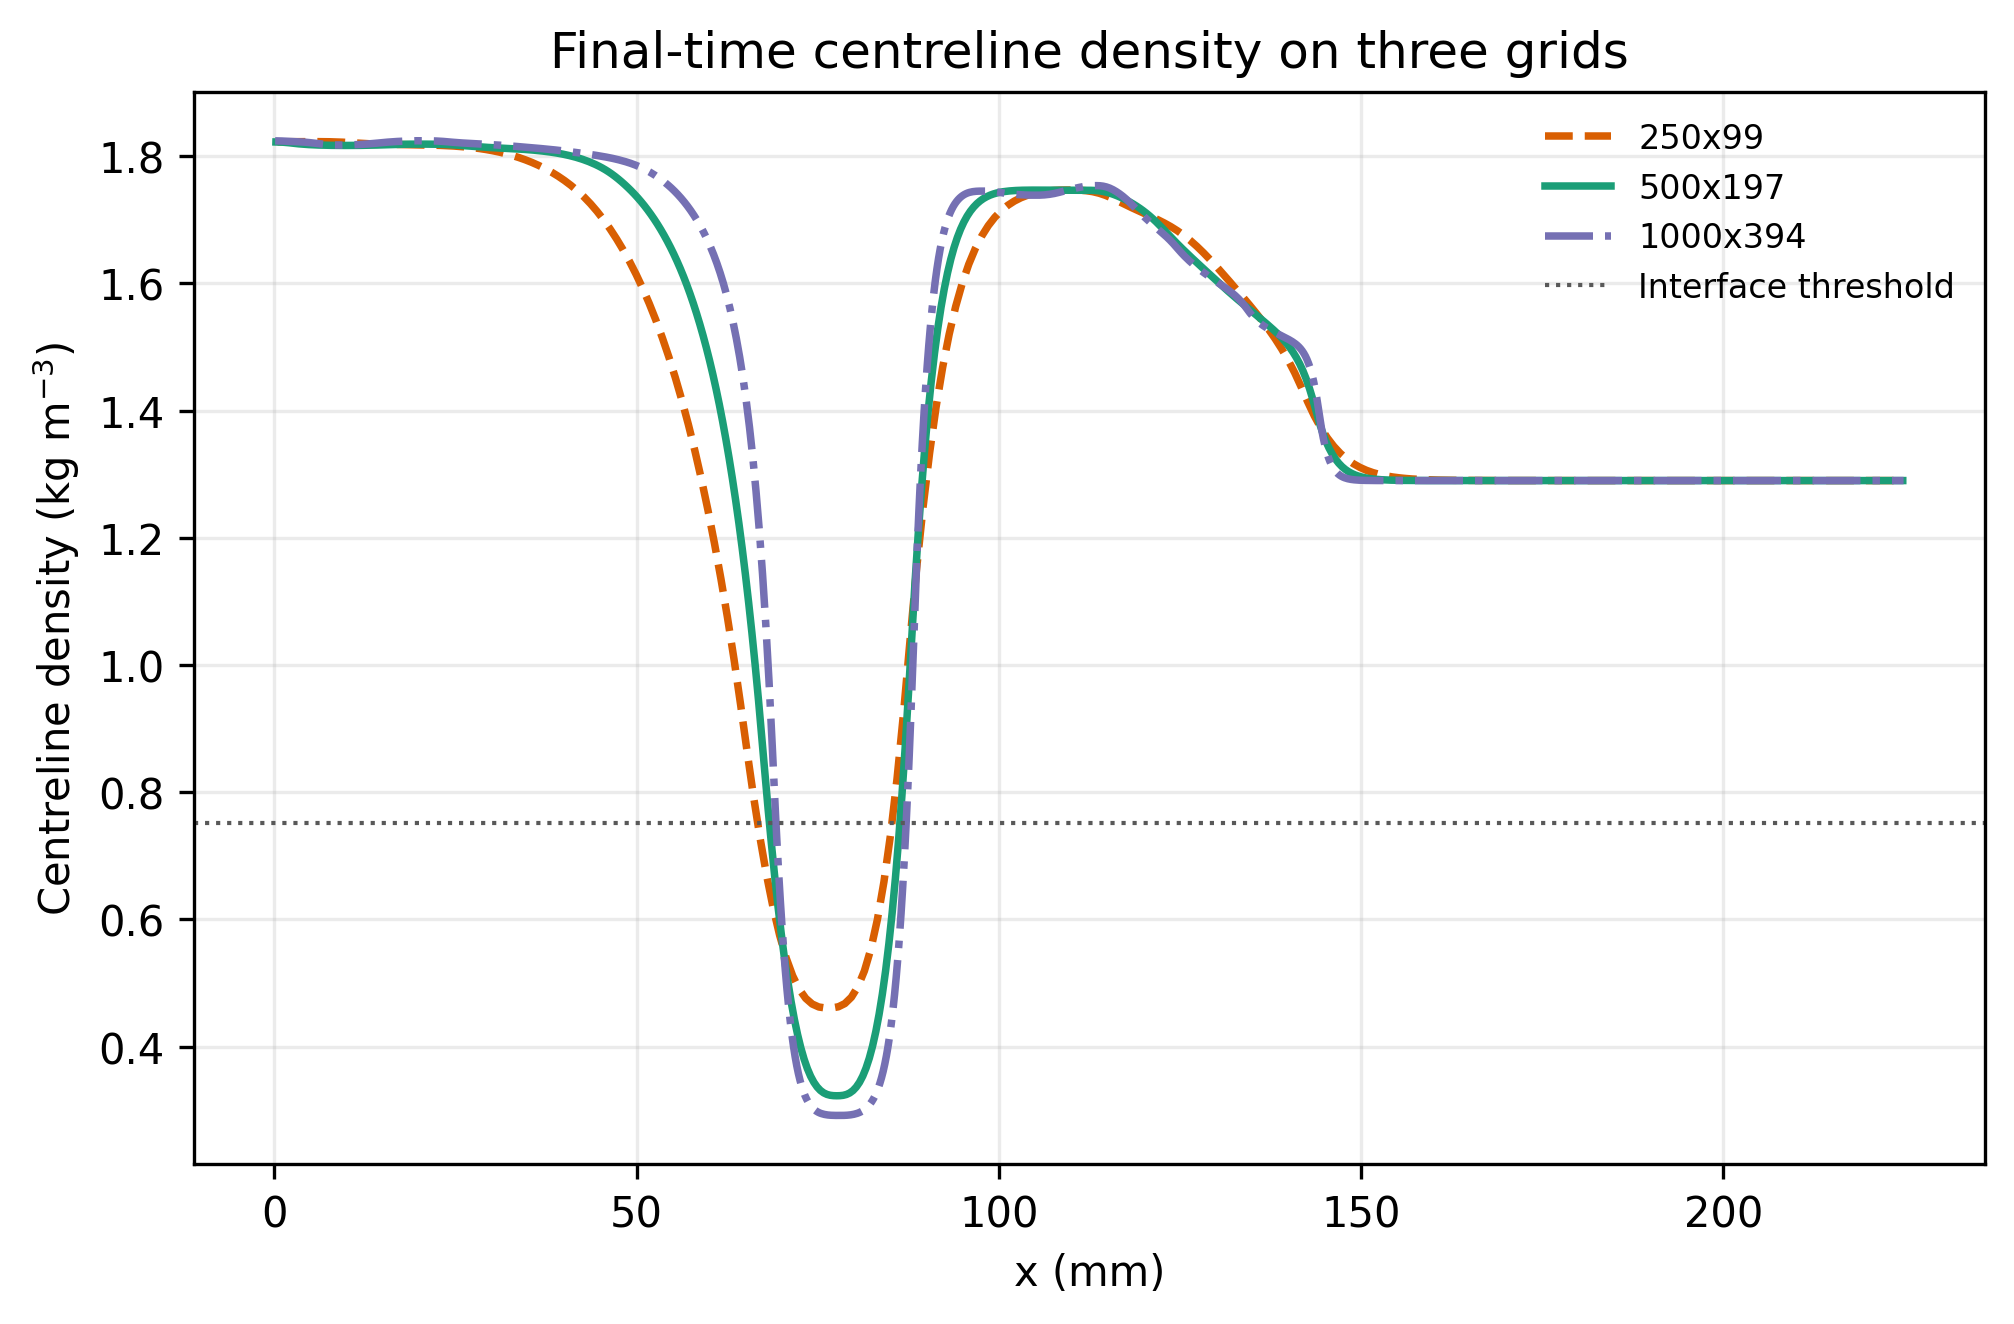
\includegraphics[width=\columnwidth]{figures/Figure_1_grid_sensitivity_density.png}
}{
  \fbox{\parbox[c][5.2cm][c]{0.95\columnwidth}{\centering Placeholder for final-time centreline density on three grids.}}
}
\caption{Final-time centreline density on three grids. The production and fine grids are close in interface location and helium-core depth, while the coarse grid is visibly more diffusive. The figure corresponds to the three-level self-convergence discussion in the text.}
\label{fig:grid_sensitivity}
\end{figure}

\begin{table}[t]
\centering
\caption{Richardson/GCI summary for final-time centreline interface positions. The estimates are scalar diagnostics only; they are not claimed as full-field asymptotic convergence.}
\label{tab:interface_richardson}
\small
\setlength{\tabcolsep}{3pt}
\begin{tabular}{lcccc}
\toprule
Interface & $p$ & Ext. (mm) & Prod. err. & AR \\
\midrule
Left & 0.840 & 70.39 & 2.9\% & 1.013 \\
Right & 0.342 & 90.46 & 4.5\% & 1.010 \\
\bottomrule
\end{tabular}
\normalsize
\end{table}

These checks do not constitute a full asymptotic accuracy study, but they are strong enough to support the later regression comparisons and to justify treating the production grid as numerically useful rather than arbitrary.

It is also worth noting what is \emph{not} used as the main validation diagnostic. Global mass, momentum, and energy conservation are less informative here than they would be in a closed-domain test because the assignment requires transmissive boundaries on all sides. Once waves approach the edges of the domain, physically correct behaviour allows mass and energy to leave the computational box. For that reason, symmetry, positivity, and 1D consistency are more useful diagnostics for this benchmark than a raw conservation tally over the full runtime.

\section{Benchmark Comparison and Physical Discussion}

The central physical comparison is with the Mach 1.22 case in Bagabir and Drikakis~\cite{bagabir2001}. Their paper reports density contours at several dimensionless times and describes the early formation of regular reflection and twin regular reflection--refraction, followed by bubble expansion, a kidney-shaped deformation, and a re-entrant jet that rolls into a vortex.

The present simulation reaches a physical time of $3.0 \times 10^{-4}~\mathrm{s}$, or approximately $t = 4.85$. This places the production snapshot near the published $t = 4.6$ contour. Figure~\ref{fig:densitypressure} shows a strongly deformed low-density helium region that has folded into a broad C- or kidney-shaped structure. The ambient shock remains visible to the right as a nearly vertical compression front, while the internal transmitted structure has moved more rapidly through the helium, consistent with the higher sound speed inside the bubble. This is the same broad behaviour described in the reference study.

\begin{figure*}[t]
\centering
\IfFileExists{figures/Figure_2_production_fields.png}{
  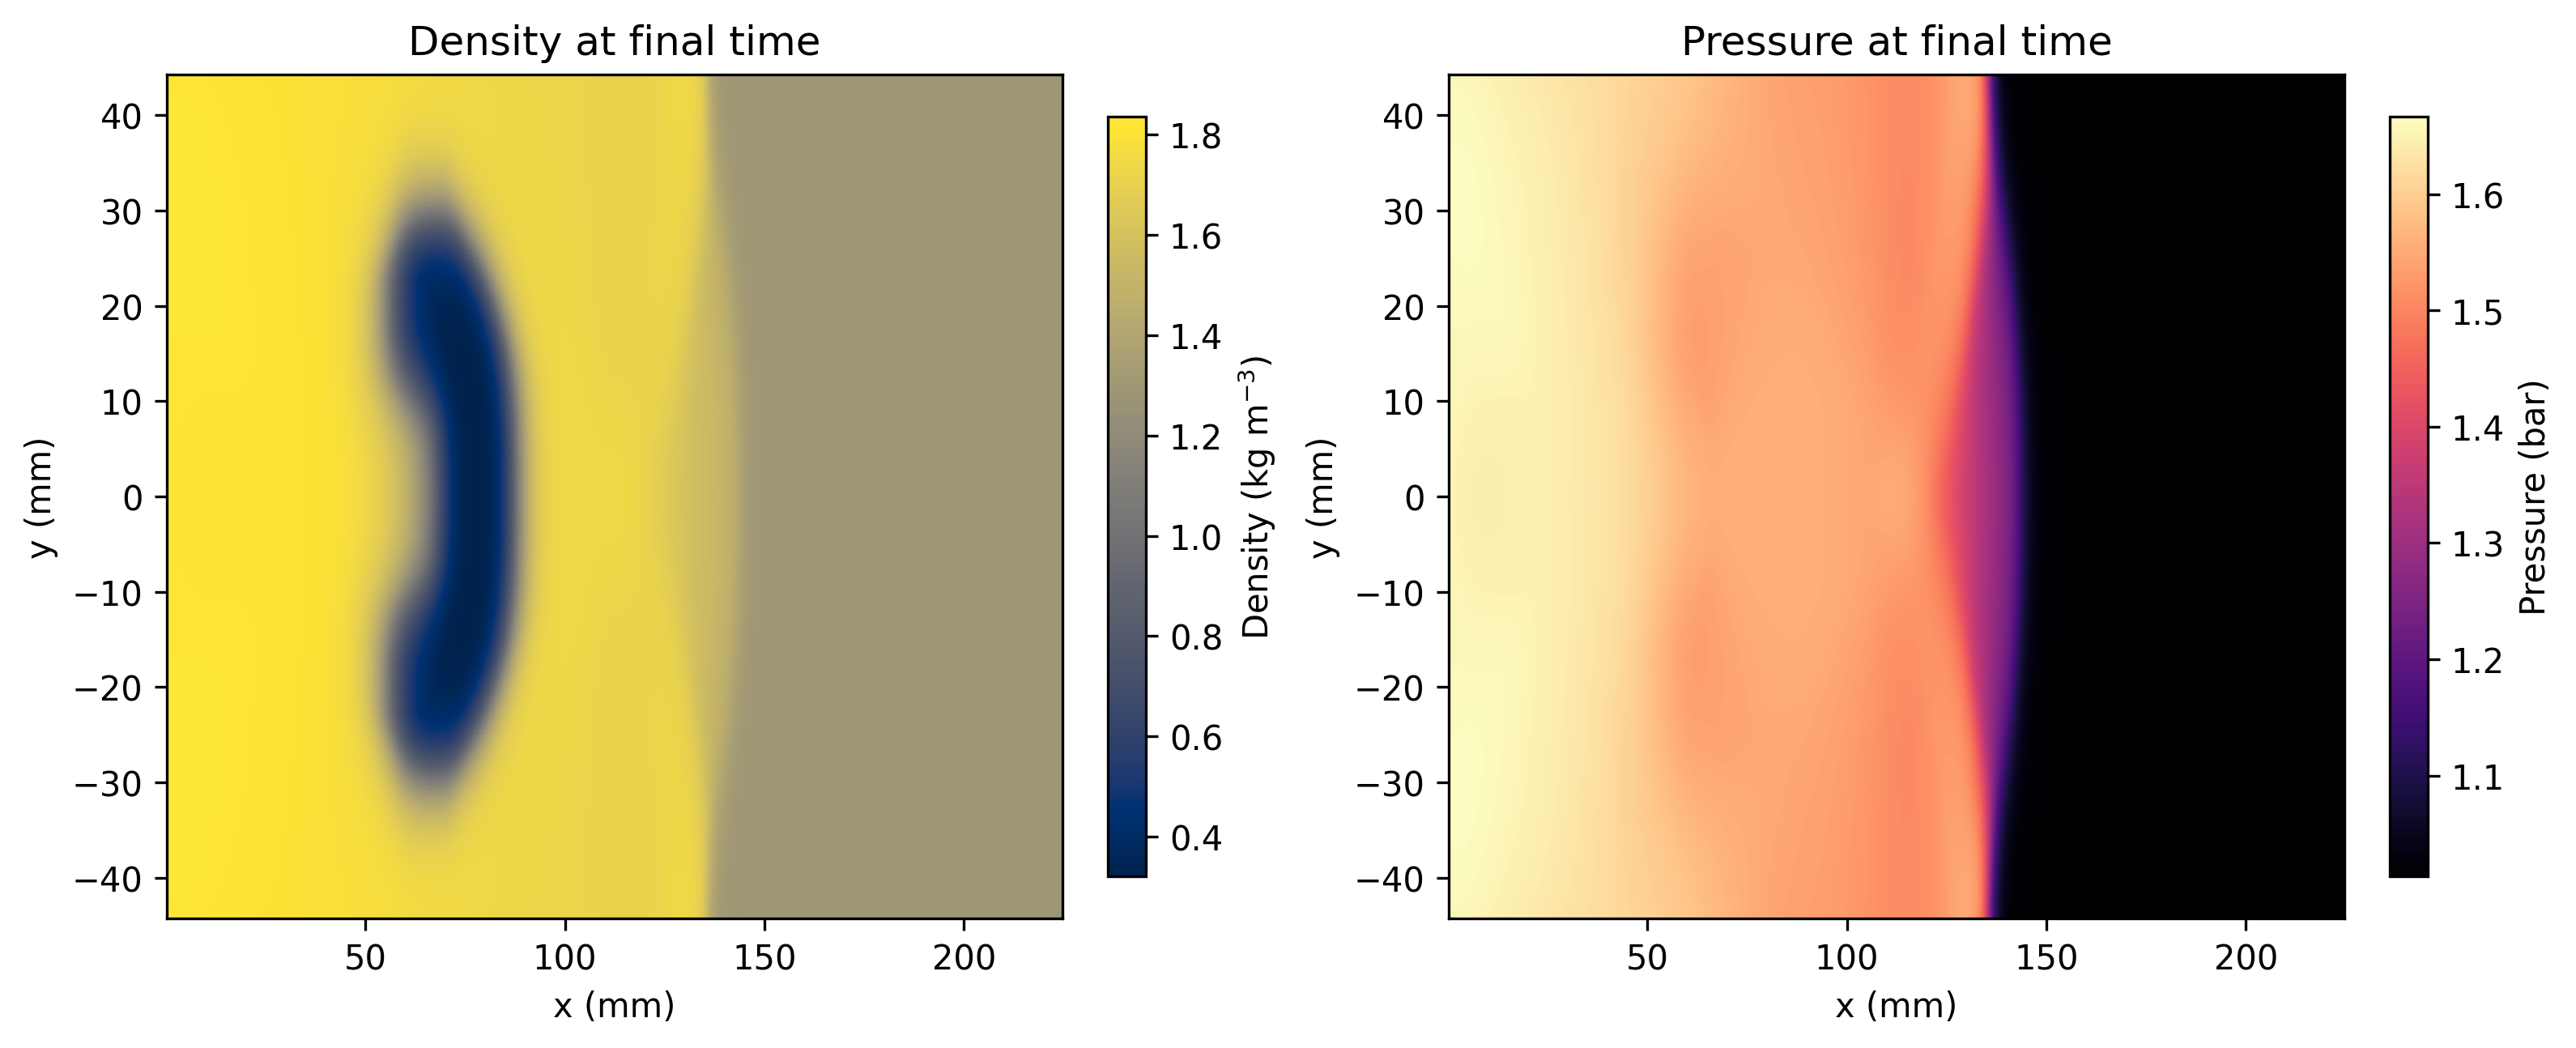
\includegraphics[width=\textwidth]{figures/Figure_2_production_fields.png}
}{
  \fbox{\parbox[c][5.2cm][c]{0.96\textwidth}{\centering Placeholder for density and pressure fields from the production baseline.}}
}
\caption{Production baseline at $500 \times 197$ and $T = 3.0 \times 10^{-4}~\mathrm{s}$ ($t \approx 4.85$ in the nondimensionalization of Bagabir and Drikakis~\cite{bagabir2001}). Left: density. Right: pressure. Both panels are rendered from the solver output with physical axes and colour bars.}
\label{fig:densitypressure}
\end{figure*}

A more direct comparison is possible from the benchmark time series. The centreline density was post-processed with the threshold $\rho = 0.752~\mathrm{kg\,m^{-3}}$, halfway between the initial air and helium densities. This is a deliberately reduced diagnostic: it compresses a deforming two-dimensional interface into two scalar positions, so it cannot reproduce full contour topology, but it does provide a reproducible comparison of interface-motion scale. To avoid relying on a pure eye-estimate, the paper figures were digitized from calibrated image crops. The late-time portion of Fig.~3 was read at the same times sampled in the numerical benchmark series wherever the jet and downstream curves are recoverable cleanly. Over that window, the numerical jet proxy is low by a mean absolute difference of about $1.9$~mm (maximum $3.1$~mm), while the downstream proxy is low by about $3.7$~mm on average (maximum $4.2$~mm). At $t \approx 3.00$, the two recoverable centreline thresholds in the present solver reach $34.05$~mm and $60.46$~mm. Independent digitized points from Figs.~3 and~12b of Bagabir and Drikakis then give jet displacements of $35.5$--$36.4$~mm and downstream displacements of $63.0$--$63.8$~mm. The present solver is therefore low by about $1.45$--$2.35$~mm for the jet proxy and $2.54$--$3.34$~mm for the downstream proxy, corresponding to differences of roughly $4$--$7\%$. Those offsets are larger than the local digitization uncertainty alone, so they should be read as evidence of the correct interface-motion scale rather than as near-exact contour agreement. The consistent low bias is physically plausible for a full-bubble calculation with different boundaries and a deliberately diffusive FORCE flux. A $45$--$55\%$ threshold sweep between the helium and air densities moves the $t \approx 3$ jet proxy only from $33.63$ to $34.50$~mm and the downstream proxy from $60.10$ to $60.79$~mm; the late-time Fig.~3 mean absolute differences remain within $1.45$--$2.32$~mm for the jet and $3.37$--$4.06$~mm for the downstream proxy. The benchmark interpretation is therefore not an artefact of a single threshold choice. Figure~\ref{fig:interface_tracking} shows the full trajectory of the numerical proxies together with the digitized paper points. The left threshold is best interpreted as a jet proxy after the interface folds over; the outer upstream interface itself is not cleanly represented by a single centreline threshold in the present full-bubble calculation.

\begin{figure}[t]
\centering
\IfFileExists{figures/Figure_3_interface_tracking.png}{
  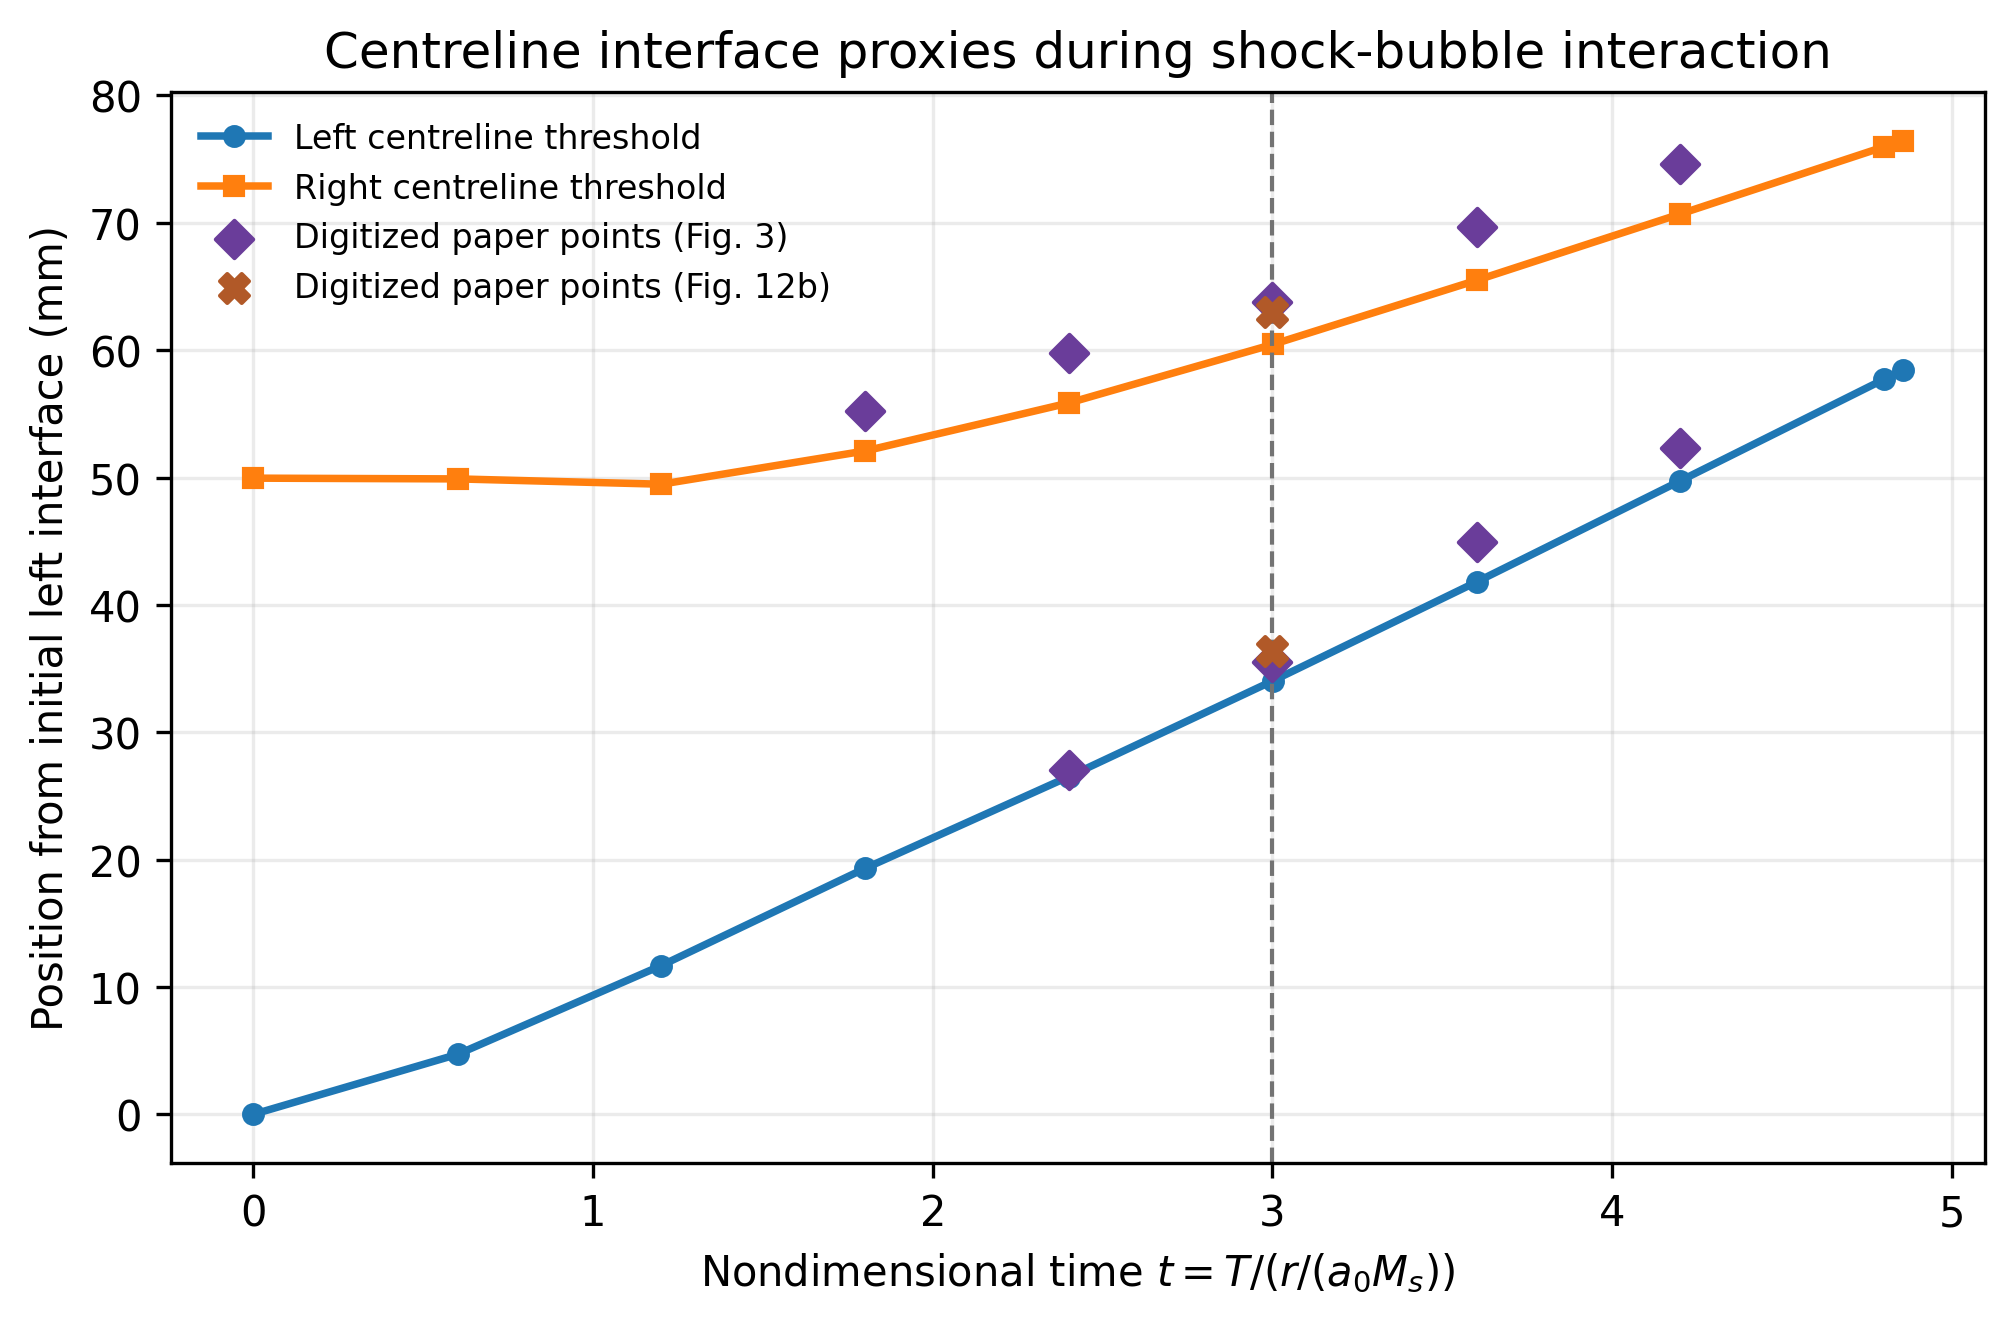
\includegraphics[width=\columnwidth]{figures/Figure_3_interface_tracking.png}
}{
  \fbox{\parbox[c][5.2cm][c]{0.95\columnwidth}{\centering Placeholder for centreline interface-proxy trajectories.}}
}
\caption{Centreline interface proxies obtained from the density threshold $\rho = 0.752~\mathrm{kg\,m^{-3}}$. The reference markers combine late-time digitized points from the Fig.~3 space--time diagram and an independent $t \approx 3.0$ cross-check from Fig.~12b of Bagabir and Drikakis~\cite{bagabir2001}.}
\label{fig:interface_tracking}
\end{figure}

The most convincing point of agreement is therefore still morphological, but it is no longer only qualitative. In both the paper and the present solver, the weak shock passes more quickly through the helium than through the surrounding air, the bubble flattens and folds into a kidney-like shape, and the centre of the bubble develops a jet that drives later vortex formation. The velocity fields support the same interpretation: the streamwise velocity shows a fast jet-like core through the bubble, while the transverse velocity reveals antisymmetric lobes above and below the centreline. Because the simulation computes the full bubble with transmissive top and bottom boundaries, this pattern is cleaner and more symmetric than the half-domain, wall-bounded configuration in the paper.

The comparison still has to be framed carefully. The reference paper shows a contour sequence over several times, whereas the present run is represented mainly by one full-resolution snapshot, a short time series, and the associated validation outputs. The report therefore supports careful agreement in morphology and interface-motion scale, but not detailed claims about every intermediate reflection pattern or near-exact contour replication. The systematic low bias in the scalar proxies is also physically interpretable: different boundary conditions and the deliberately diffusive FORCE flux both tend to soften sharp interface motion and delay the threshold crossings used here as reduced diagnostics.

\section{Performance Results}

The performance results are split into a full-resolution compiler study, a reduced-grid structural study, and a repeated full-grid structural study. Compiler flags were tested directly on the full $500 \times 197$ production case. The reduced-grid structural study was kept as a cheap screening step, but its smaller penalties are interpreted alongside the repeated full-grid campaign rather than in isolation.

The compiler study used one warmup and nine timed repetitions per variant on the production benchmark, and Table~\ref{tab:compiler} reports sample standard deviations and 95\% confidence-interval half-widths as well as means. The baseline build with \texttt{-O3 -march=native} completed in $20.22 \pm 0.26$~s. Generic \texttt{-O3} required $20.14 \pm 0.24$~s, \texttt{-O2} required $20.21 \pm 0.48$~s, and \texttt{-O1} required $21.57 \pm 0.32$~s. All variants reproduced the baseline solution exactly at recorded output precision. The practical conclusion is therefore deliberately cautious: on this Apple M4 system, avoiding low optimisation levels matters clearly, but \texttt{-O3 -march=native}, generic \texttt{-O3}, and \texttt{-O2} are effectively tied within the observed dispersion. Generic \texttt{-O3} has the lowest mean time and is also the cleanest portable reference build, whereas \texttt{-march=native} does not show a decisive advantage here.

\begin{table*}[t]
\centering
\caption{Compiler study on the full $500 \times 197$ benchmark. Each variant uses one warmup and nine timed runs; ratios are based on mean wall time.}
\label{tab:compiler}
\begin{tabular}{lcccccl}
\toprule
Variant & Mean time (s) & Std. dev. (s) & 95\% CI (s) & Time / baseline & Density $\ell_\infty$ error & Build \\
\midrule
Baseline & 20.2223 & 0.2566 & 0.1677 & 1.000 & 0.0 & \texttt{-O3 -march=native} \\
\texttt{-O1} & 21.5709 & 0.3242 & 0.2118 & 1.067 & 0.0 & \texttt{-O1} \\
\texttt{-O2} & 20.2149 & 0.4819 & 0.3148 & 1.000 & 0.0 & \texttt{-O2} \\
Generic \texttt{-O3} & 20.1428 & 0.2366 & 0.1546 & 0.996 & 0.0 & \texttt{-O3} \\
\bottomrule
\end{tabular}
\end{table*}

The reduced-grid structural study, summarized in Table~\ref{tab:structural}, is useful mainly as a screening experiment. Replacing fixed-size state storage with \texttt{std::vector} is again the clearest negative result, giving a slowdown of about $18.2\times$ on the reduced grid, and disabling reconstruction caching is again the next largest effect at about $1.66\times$. By contrast, the smaller structural differences essentially disappear into the short-benchmark dispersion: state-by-value, grid-by-value, and cache-unfriendly traversal all lie within about $2.5\%$ of baseline, and two of them are nominally faster than baseline on mean time. The reduced-grid study should therefore be read as strong evidence only for the large structural effects and as a cheap screening step before the full-grid campaign. In all cases the recorded numerical output remained unchanged, so the effect is on runtime only, not on the computed solution.

The repeated full-grid structural study in Table~\ref{tab:structural_fullgrid} is the authoritative source for the final structural conclusions. It shows that state-by-value, grid-by-value, and cache-unfriendly traversal are all only about $0.9$--$1.3\%$ slower than baseline, with overlapping confidence intervals; on this machine they are best described as modest secondary effects rather than sharply separated penalties. Disabling reconstruction caching remains a large penalty at about $1.67\times$. A separate repeated full-grid campaign was then run for the pathological \texttt{std::vector} state variant, using a paired baseline in the same round-robin schedule: it gives $382.04 \pm 1.32$~s against $19.97 \pm 0.26$~s, a slowdown of about $19.1\times$. This is materially stronger evidence than the earlier combination of reduced-grid trends and one-off confirmation checks.

\begin{table*}[t]
\centering
\caption{Structural-variant study on the reduced $160 \times 63$ benchmark. Each variant uses one warmup and nine timed runs; ratios are based on mean wall time.}
\label{tab:structural}
\small
\setlength{\tabcolsep}{4pt}
\begin{tabular}{>{\raggedright\arraybackslash}p{3.1cm}ccccc>{\raggedright\arraybackslash}p{3.8cm}}
\toprule
Variant & Mean time (s) & Std. dev. (s) & 95\% CI (s) & Time / baseline & Pressure $\ell_\infty$ error & Interpretation \\
\midrule
Baseline & 0.6036 & 0.0464 & 0.0303 & 1.000 & 0.0 & Cache-friendly fixed-size state storage \\
\texttt{std::vector} state & 11.0088 & 0.2016 & 0.1317 & 18.237 & 0.0 & Dynamic container overhead dominates \\
State by value & 0.5884 & 0.0044 & 0.0029 & 0.975 & 0.0 & Effect too small to separate cleanly here \\
Grid by value & 0.6027 & 0.0359 & 0.0234 & 0.999 & 0.0 & Effect too small to separate cleanly here \\
Cache-unfriendly access & 0.6000 & 0.0256 & 0.0167 & 0.994 & 0.0 & Effect too small to separate cleanly here \\
No reconstruction cache & 1.0021 & 0.1026 & 0.0670 & 1.660 & 0.0 & Expensive repeated interface work \\
\bottomrule
\end{tabular}
\normalsize
\end{table*}

\begin{table*}[t]
\centering
\caption{Repeated production-grid structural study on $500 \times 197$. Each variant uses one warmup and nine timed runs, except the \texttt{std::vector} row, which comes from a separate one-warmup, three-timed-run paired campaign with its own baseline. Ratios are based on mean wall time within each campaign.}
\label{tab:structural_fullgrid}
\small
\setlength{\tabcolsep}{3pt}
\begin{tabular}{>{\raggedright\arraybackslash}p{2.8cm}ccccc}
\toprule
Variant & Mean time (s) & Std. dev. (s) & 95\% CI (s) & Time/base & $\rho$ $\ell_\infty$ \\
\midrule
Baseline & 20.0898 & 0.1937 & 0.1265 & 1.000 & 0.0 \\
\texttt{std::vector} state & 382.0406 & 1.3219 & 1.4959 & 19.135 & 0.0 \\
State by value & 20.3471 & 0.3032 & 0.1981 & 1.013 & 0.0 \\
Grid by value & 20.3005 & 0.3511 & 0.2294 & 1.010 & 0.0 \\
Cache-unfriendly access & 20.2698 & 0.1740 & 0.1137 & 1.009 & 0.0 \\
No reconstruction cache & 33.5086 & 0.2667 & 0.1742 & 1.668 & 0.0 \\
\bottomrule
\end{tabular}
\normalsize
\end{table*}

The most important observation from all of the performance evidence is that every tested variant matched the baseline at recorded output precision, including the repeated full-grid \texttt{std::vector} study. The optimisation study therefore supports faster implementation without evidence of altered numerics.

The performance study supports four practical lessons. First, sensible compiler settings are a necessary baseline, but on this machine the dominant compiler lesson is simply to avoid low optimisation levels; among the optimized builds tested, the differences are too small to support a strong ranking beyond saying that generic \texttt{-O3} is the cleanest portable reference. Second, for a four-component Euler state, inline fixed-size storage is decisively better than dynamic per-state storage. Third, avoiding unnecessary copying and preserving locality help, but those penalties are modest secondary effects at full scale here. Fourth, caching intermediate reconstructed states is a broadly useful optimisation because it removes redundant work without changing the numerical update. Taken together, the experiments show a clear hierarchy of effects: once a reasonable optimized build is chosen, memory layout and explicit reuse matter far more than marginal compiler tuning.

\section{Limitations and Further Work}

Although the current solver meets the core assignment goals, several limitations should be stated explicitly. The first is numerical accuracy. A SLIC/FORCE formulation with a minmod limiter is robust but diffusive. It reproduces the main structures of the Mach 1.22 benchmark, yet it does not provide the sharpest possible interface representation. Closely related to this, the report now includes a genuine three-level self-convergence study, a planar-shock plateau reference check, and cautious Richardson/GCI uncertainty indicators for both scalar interface positions and field norms, but it still stops short of a fuller Richardson-style analysis over more grids and diagnostics. The observed full-field orders of about $0.4$--$0.8$ are plausible for a shock-dominated problem, but a stronger dissertation-level submission would still add more systematic convergence evidence.

The second limitation is the use of a single ideal-gas model. This is consistent with the assignment and with the simplified setup discussed in the reference literature, but it does not represent thermal equilibrium across the air--helium interface. For the present report, this is acceptable because the emphasis is on large-scale morphology and performance. For a more physically complete study, one would need a multi-species or variable-$\gamma$ model and probably a sharper interface treatment.

The third limitation concerns the remaining scope gaps in the performance and benchmark evidence. The repeated full-grid structural campaign has removed the earlier one-off timing weakness, but penalties of only a few per cent remain machine-dependent and should not be over-generalised beyond the present platform. The benchmark comparison has also been strengthened materially, yet it still digitizes only a partial subset of the published information. Natural extensions would therefore be a sharper flux or limiter, a broader grid study, more extensive timing campaigns if one wanted sub-per-cent performance resolution, and fuller digitization of the benchmark paper. Any such extension would need to keep the same regression discipline used here, so that sharper numerics or more aggressive optimisation remain demonstrably controlled.

\section{Conclusions}

This project set out to build a numerically credible and computationally efficient 2D Euler solver for shock interaction with a helium bubble, and to use that solver as a test bed for performance-oriented code experiments. Both aims were met. The final C++ code runs the full assignment benchmark on a $500 \times 197$ grid with transmissive boundaries in about $20$~s on a single Apple M4 core using Apple Clang 17. The baseline passes invariance, symmetry, positivity, and finiteness checks, gives sub-$1\%$ planar-shock plateau errors away from the numerically broadened shock, shows plausible low-order self-convergence, and reproduces the main Mach 1.22 morphology with a modest systematic low bias in interface position relative to Bagabir and Drikakis. It does not claim high-fidelity contour replication of the reference paper; what it does support is an assignment-level benchmark reproduction under the simplified single-gas SLIC/FORCE assumptions. Against the central questions posed by the assignment, the evidence now supports both a credible numerical baseline and a clear ranking of the implementation choices that most affect single-core cost.

The optimal code structure supported by the data is a flat contiguous grid with ghost cells in the same storage, fixed-size inline Euler states, in-place sweeps, pass-by-reference helper calls, regular traversal, and cached reconstructed states. Replacing fixed-size state storage with \texttt{std::vector} is overwhelmingly expensive: repeated full-grid runs required about $19.1\times$ the paired baseline runtime. Disabling reconstruction caching remains a large penalty even at full scale at about $1.67\times$. By contrast, the penalties for by-value helpers and cache-unfriendly traversal are only about $0.9$--$1.3\%$ on the repeated full-grid study and are best treated as modest secondary effects on this machine. These are runtime effects only: all tested variants preserved the recorded numerical output of the baseline.

The build story is more nuanced than the structural story. Generic \texttt{-O3} has the lowest mean wall time in the repeated compiler campaign, but generic \texttt{-O3}, \texttt{-O3 -march=native}, and \texttt{-O2} are effectively tied within the observed dispersion, whereas \texttt{-O1} is clearly slower. The cleanest recommendation is therefore to use generic \texttt{-O3} as the portable reference build and to treat \texttt{-march=native} as an optional machine-specific local tweak rather than a decisive optimisation. The most transferable lessons are the structural ones: contiguous storage, avoiding dynamic per-state allocation, avoiding unnecessary copies, and reusing reconstructed data. Within those limits, the evidence supports a more specific judgement: once a reasonable optimized build is chosen, the dominant remaining costs come from data movement and redundant reconstruction work, not from marginal compiler tuning alone.

That distinction between transferable and machine-specific optimizations matters beyond this benchmark. Flat contiguous storage, fixed-size inline states, avoiding unnecessary copies, and reusing reconstructed data should remain useful in larger finite-volume or AMR-style codes, because those frameworks still spend most of their time inside cell-update kernels. By contrast, the identity of the fastest compiler and the exact benefit of \texttt{-march=native} are more machine-dependent. The report can therefore support a clear recommendation for the local best code structure and a portable reference build, while showing that the most valuable optimizations are the ones that reduce memory traffic and redundant work without changing the discretization.

\begin{thebibliography}{99}

\bibitem{bagabir2001}
A.~Bagabir and D.~Drikakis,
Mach number effects on shock-bubble interaction,
\emph{Shock Waves}, 11 (2001), pp.~209--218.

\bibitem{picone1988}
J.~M. Picone and J.~P. Boris,
Vorticity generation by shock propagation through bubbles in a gas,
\emph{Journal of Fluid Mechanics}, 189 (1988), pp.~23--51.

\bibitem{quirk1996}
J.~J. Quirk and S.~Karni,
On the dynamics of a shock-bubble interaction,
\emph{Journal of Fluid Mechanics}, 318 (1996), pp.~129--163.

\bibitem{haas1987}
J.~F. Haas and B.~Sturtevant,
Interaction of weak shock waves with cylindrical and spherical gas inhomogeneities,
\emph{Journal of Fluid Mechanics}, 181 (1987), pp.~41--76.

\bibitem{toro2009}
E.~F. Toro,
\emph{Riemann Solvers and Numerical Methods for Fluid Dynamics},
3rd ed., Springer, Berlin, 2009.

\bibitem{toro1994}
E.~F. Toro, M.~Spruce and W.~Speares,
Restoration of the contact surface in the HLL-Riemann solver,
\emph{Shock Waves}, 4 (1994), pp.~25--34.

\bibitem{vanleer1979}
B.~van Leer,
Towards the ultimate conservative difference scheme. V. A second-order sequel to Godunov's method,
\emph{Journal of Computational Physics}, 32 (1979), pp.~101--136.

\bibitem{harten1983}
A.~Harten, P.~D. Lax and B.~van Leer,
On upstream differencing and Godunov-type schemes for hyperbolic conservation laws,
\emph{SIAM Review}, 25 (1983), pp.~35--61.

\end{thebibliography}

\end{document}
